% =====================================================================
%  Academic paper template  —  single-column article class
%  Compile:  bash scripts/compile.sh paper-template.tex
%  Uses natbib + bibtex (no biber needed). Times-like fonts.
% =====================================================================
\documentclass[11pt,a4paper]{article}

% --- encoding & fonts ---
\usepackage[T1]{fontenc}
\usepackage[utf8]{inputenc}
\usepackage{mathptmx}        % Times-like text + math (classic paper look)
\usepackage{microtype}       % subtle spacing fixes; fewer overfull boxes

% --- layout ---
\usepackage[margin=1in]{geometry}
\usepackage{setspace}

% --- math ---
\usepackage{amsmath,amssymb,mathtools}
\usepackage{amsthm}
\usepackage{siunitx}         % \SI{3.2}{\meter}, aligned numeric table columns

% --- figures & tables ---
\usepackage{graphicx}
\usepackage{booktabs}        % \toprule \midrule \bottomrule (never use \hline)
\usepackage{caption}
\usepackage{subcaption}      % side-by-side subfigures
\usepackage{tikz}
\usepackage{pgfplots}
\pgfplotsset{compat=1.18}

% --- algorithms ---
\usepackage{algorithm}
\usepackage{algpseudocode}

% --- bibliography & links (load hyperref last, cleveref after it) ---
\usepackage[numbers,sort&compress]{natbib}
\usepackage[hidelinks]{hyperref}
\usepackage{cleveref}        % \cref{fig:x} -> "Fig. 1", \cref{eq:y} -> "Eq. (2)"

% --- theorem environments ---
\newtheorem{theorem}{Theorem}
\newtheorem{definition}{Definition}

\title{\bfseries A Concise Template for Academic Papers}
\author{First Author\thanks{Corresponding author: first@example.edu} \and Second Author}
\date{\today}

\begin{document}
\maketitle

\begin{abstract}
\noindent
This is the abstract: one paragraph stating the problem, what you did, and the
headline result. Keep it self-contained and free of citations and undefined
acronyms. A reader should grasp the contribution from these few sentences alone.
\end{abstract}

% -------------------------------------------------------------------
\section{Introduction}
\label{sec:intro}

State the problem and why it matters, summarise prior work, and list your
contributions. Cite sources with \citet{einstein1905} for in-text mentions and
\citep{knuth1984} for parenthetical ones. Refer to floats with \cref{fig:plot}
and \cref{tab:results} — \texttt{cleveref} inserts the right word and number,
so never hard-code ``Figure 1''.

% -------------------------------------------------------------------
\section{Method}
\label{sec:method}

Define notation in a \texttt{definition} and key claims in a \texttt{theorem}.

\begin{definition}[Loss]
We minimise the loss $\mathcal{L}(\theta)=\frac{1}{n}\sum_{i=1}^{n} \ell(f_\theta(x_i), y_i)$.
\end{definition}

Display equations get a label so they can be referenced as \cref{eq:update}:
\begin{equation}
  \theta_{t+1} = \theta_t - \eta \, \nabla_\theta \mathcal{L}(\theta_t).
  \label{eq:update}
\end{equation}

\begin{algorithm}[ht]
\caption{Gradient descent}
\label{alg:gd}
\begin{algorithmic}[1]
  \State \textbf{Input:} learning rate $\eta$, steps $T$, init $\theta_0$
  \For{$t = 0$ to $T-1$}
    \State $\theta_{t+1} \gets \theta_t - \eta\,\nabla_\theta \mathcal{L}(\theta_t)$
  \EndFor
  \State \textbf{return} $\theta_T$
\end{algorithmic}
\end{algorithm}

% -------------------------------------------------------------------
\section{Results}
\label{sec:results}

% --- A figure from an external image file ---------------------------
% Replace example-image-a with your own file (PDF/PNG/JPG). width=\linewidth
% guarantees it never spills past the text margin.
\begin{figure}[ht]
  \centering
  \includegraphics[width=0.7\linewidth]{example-image-a}
  \caption{An externally supplied figure. Use \texttt{width=\textbackslash linewidth}
           (or a fraction of it) so the image always fits the column.}
  \label{fig:image}
\end{figure}

% --- A vector figure drawn in LaTeX (scales perfectly, no image file) --
\begin{figure}[ht]
  \centering
  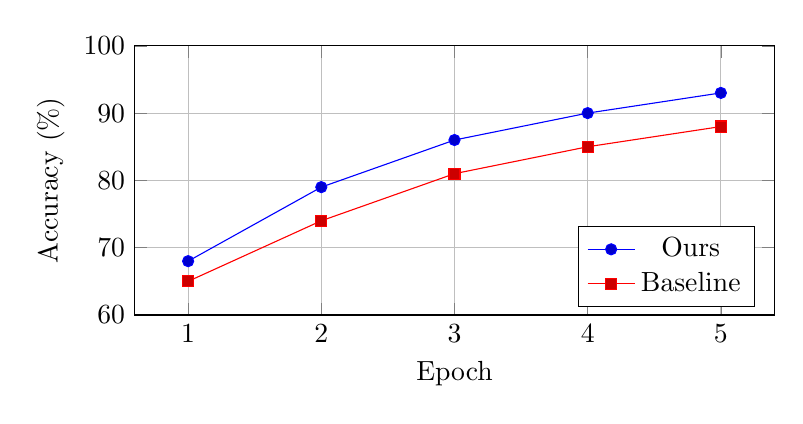
\begin{tikzpicture}
    \begin{axis}[
        width=0.8\linewidth, height=5cm,
        xlabel={Epoch}, ylabel={Accuracy (\%)},
        legend pos=south east, grid=major,
        ymin=60, ymax=100]
      \addplot coordinates {(1,68)(2,79)(3,86)(4,90)(5,93)};
      \addplot coordinates {(1,65)(2,74)(3,81)(4,85)(5,88)};
      \legend{Ours, Baseline}
    \end{axis}
  \end{tikzpicture}
  \caption{A plot drawn directly in LaTeX with \texttt{pgfplots}: vector output,
           consistent fonts, no external file to manage.}
  \label{fig:plot}
\end{figure}

% --- Side-by-side subfigures ---------------------------------------
\begin{figure}[ht]
  \centering
  \begin{subfigure}{0.45\linewidth}
    \includegraphics[width=\linewidth]{example-image-a}
    \caption{First view.}\label{fig:sub-a}
  \end{subfigure}\hfill
  \begin{subfigure}{0.45\linewidth}
    \includegraphics[width=\linewidth]{example-image-b}
    \caption{Second view.}\label{fig:sub-b}
  \end{subfigure}
  \caption{Two subfigures sharing one caption and counter.}
  \label{fig:subs}
\end{figure}

% --- A professional table with booktabs + siunitx -------------------
% S columns align numbers on the decimal point; booktabs rules look clean.
\begin{table}[ht]
  \centering
  \caption{Main results. \texttt{booktabs} rules + \texttt{siunitx} S columns.}
  \label{tab:results}
  \begin{tabular}{l S[table-format=2.1] S[table-format=1.3]}
    \toprule
    Method   & {Accuracy (\%)} & {Time (\si{\second})} \\
    \midrule
    Baseline & 88.0 & 1.240 \\
    Ours     & 93.2 & 0.870 \\
    \bottomrule
  \end{tabular}
\end{table}

% -------------------------------------------------------------------
\section{Conclusion}
\label{sec:conclusion}
Restate the contribution and point to future work.

% -------------------------------------------------------------------
\bibliographystyle{plainnat}   % author–year; use IEEEtran/unsrtnat as needed
\bibliography{references}

\end{document}
